%!TEX root = ../thesis.tex
\section{Introduction}

Popular online video-sharing websites such as YouTube have enabled the growth of a large community of users who share their knowledge and expertise in video tutorials. How-To videos demonstrate specific skills and procedures for tasks as varied as cooking, building a treehouse, or fixing a machine \cite{Torrey:2007he}.
These online tutorials help learners observe the manipulations and then put them into practice \cite{Torrey:2009fc}. However, in recording these videos, instructors often find it challenging to control the camera during demonstration.
%
Working with a cameraman who controls the device and viewpoints ensures that the video captures the movements that the audience would want to see, but it requires having a second person to direct the recording and work closely together with instructors. Many amateur users who mostly work alone, therefore, choose to self-record with one or more cameras. Camcorders can be set on a tripod to capture a static viewpoint, but it is hard to make sure whether users' actions are properly in frame at recording time. An alternative is to wear a head mounted camera to record what the instructors see. This may record unwanted and distractive head movements, making it difficult for the audience to watch. Additional camera views of the overall workspace might be needed to assist learners with understanding the context of demonstrated actions~\cite{Fussell:2003te}.

\begin{figure}[t]
\centering
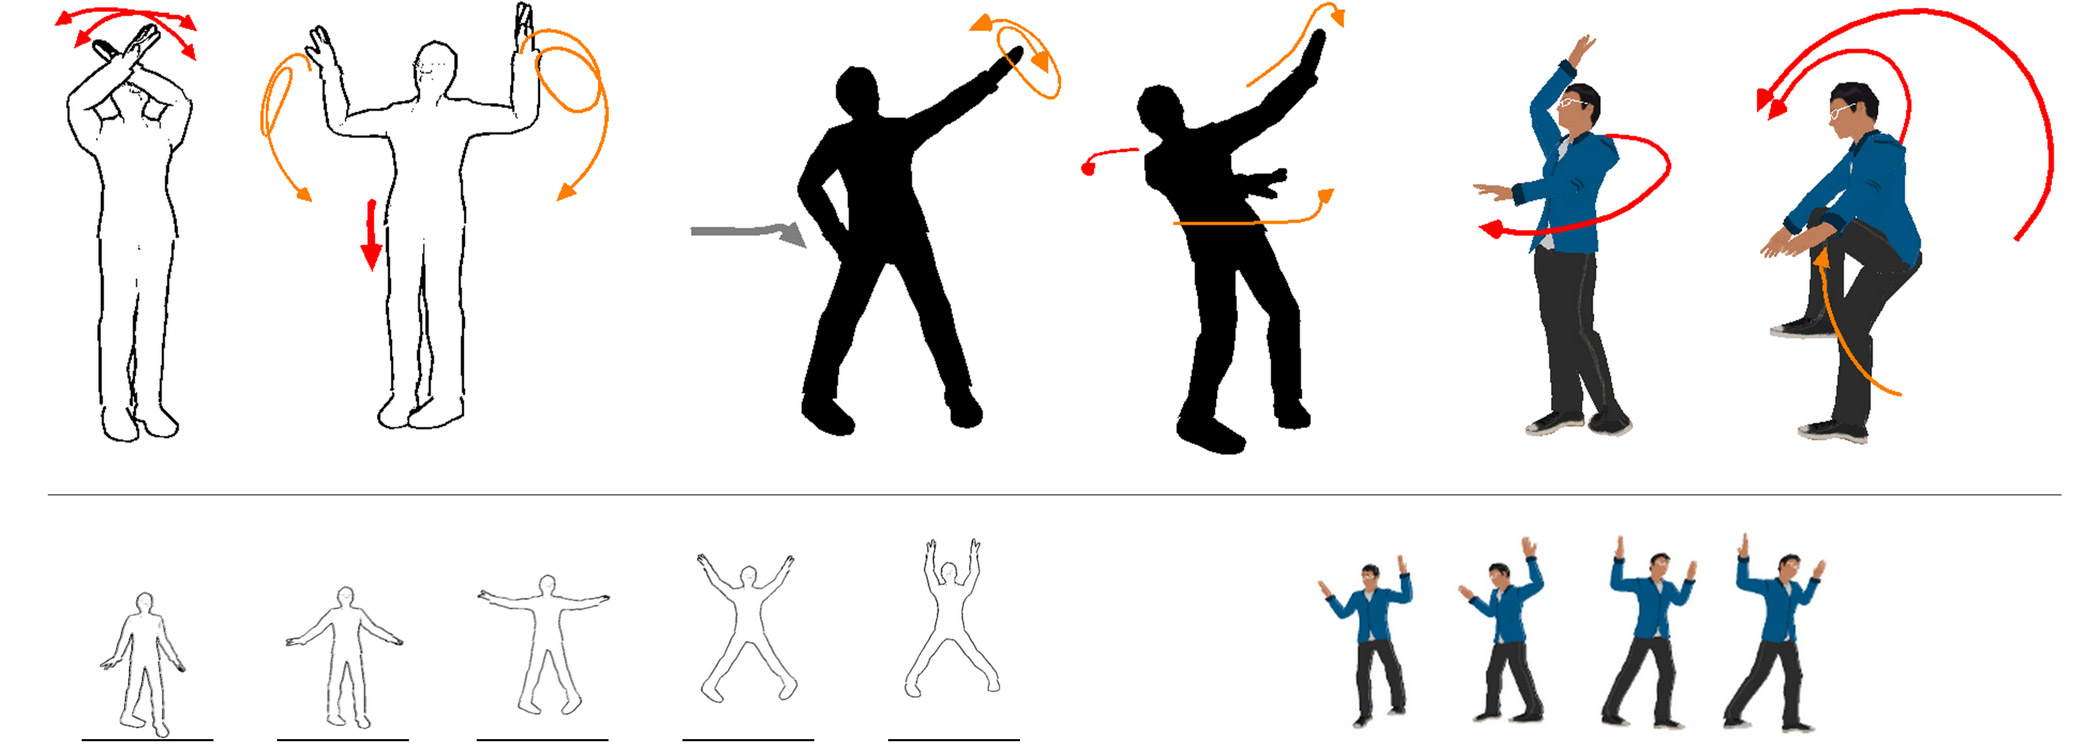
\includegraphics[height=0.25\textheight]{\kinectograph/fig/teaser}\\
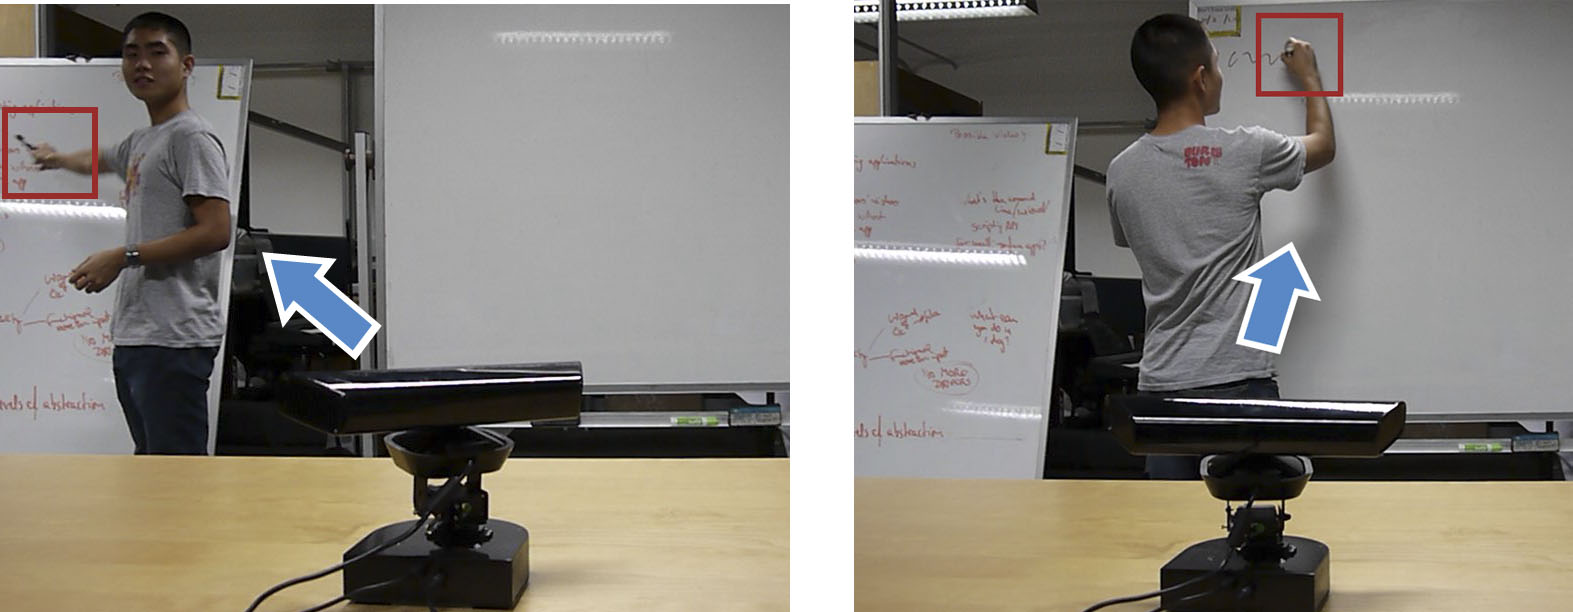
\includegraphics[height=0.22\textheight]{\kinectograph/fig/Kinectograph_following}
\caption{Kinectograph includes a Kinect camera to track user movement and a motorized dock to pan and tilt the camera so that the user (or their hand) remains centered in the recorded video. Here the device follows the user\'s hand while he is illustrating.}
\label{fig:figure1}
\end{figure}

Seeing these filming challenges, we would like to enable users to gain the flexibility of real-time camera control without requiring a dedicated camera-person. Our goal is to design a device that can automatically track and orient to film the tutorial instructors while providing lightweight manual controls. Existing video conferencing cameras and surveillance tools offer human tracking to provide full or partial automatic viewpoint control. Polycom\footnote{http://www.polycom.com/} designs video conferencing cameras that feature face recognition and voice detection to enable a group of users to talk in an office room setting. This approach assumes people's faces should be in the frame, which may not be true for instructional videos that focus on actions rather than ``talking heads.''
%
Automatic motion tracking is possible to always keep the user in view using visible markers \cite{Ranjan:2010} or wearable sensors such as infrared emitters by Swivl\footnote{http://www.swivl.com/}. However, instructors are unlikely to take such approaches to put on visible markers when demonstrating.
%
Researchers have been developing techniques to track specific targets using computer vision, including hands \cite{Ranjan:2008}, user movements \cite{Wilson:2012fb}, fast-moving objects (e.g., a Ping-Pong ball) \cite{Okumura:2011tr}, or regions in pre-defined spaces \cite{Ranjan:2007}. These usually require an expert defining heuristics of space regions or movement classifications ahead of time for the tracking program. On the contrary, we aim at proposing a new approach that does not have these issues, gives users flexibility in a home environment, and provides interactive control over the behavior of the camera tracking.
%
% TeleAdvisor assists a helper to remotely observe a physical task in real-time and provide instructions~\cite{Gurevich:2012ko}. However, the system is limited by the static camera view without automatic tracking.
%

We propose Kinectograph, a new device that enables semi-automatic camera control for users to self-direct camera orientation for demonstration tasks (Figure~\ref{fig:figure1}). Kinectograph serves as both the camera and the cameraman. It provides a motorized dock for a Kinect\footnote{http://www.xbox.com/en-US/kinect} sensor and a tablet-based user interface (separate from the camera) to switch between tracking regions at runtime based on their needs when demonstrating. Using skeleton tracking to follow the user’s movement, Kinectograph automatically pans and tilts the camera in real time. Users can define zoom regions that follow his actions to provide closeup views. Using a Kinect sensor, our system works in a common indoor setting and does not require the user to wear sensors or configure the environments. Kinectograph makes a novel contribution over the prior art in its mixed-initiative approach that offers various levels of automation and control to users at record time.

In the following section (Section \ref{kinectograph_authoring}), we describe the user experience of recording with Kinectograph. We also describe design and implementation decisions (Section \ref{kinectograph_tracking}). Finally, in Section \ref{kinectograph_study}, we review findings from a preliminary evaluation with 7 participants to study Kinectograph's usability of self-recording tutorials. All of the participants successfully created a demonstration video using our system without assistance and found it easy to interact with.

%\bjoern{I cut this out because you are missing the reference.}\new{In [insert citation here], they similarly use motors and a camera to automatically track and zooming in on users, but they do so in a conference setting. One of their system objectives is to unobtrusively track; however, our system focuses on providing enabling user's control in these tracking and zooming decisions for their DIY tutorials. In addition they only use facial and audio tracking and do not leverage the power of the kinect to do skeletal tracking.}

% Abhishek Ranjan, Jeremy Birnholtz, Rorik Henrikson, Ravin Balakrishnan, Dana Lee. (2010). Automatic camera control using unobtrusive vision and audio tracking. Proceedings of GI 2010 – the Graphics Interface Conference. p. 47-54.
%\pc{Where is the reference to the papers Bjoern sent? auto-tracking camera}
